\subsubsection{Shopping list} \label{ShoppingListSketches}

In this section the sketch of the shopping list is going to be described. The sketch is made up of two different screens, as seen in figure \ref{FinalShoppingListSketch}. One of the screens indicate the overview of the items on the shopping list, and the other screen shows the screen when something has been typed into the search bar.

\begin{figure}[H]
    \centering
    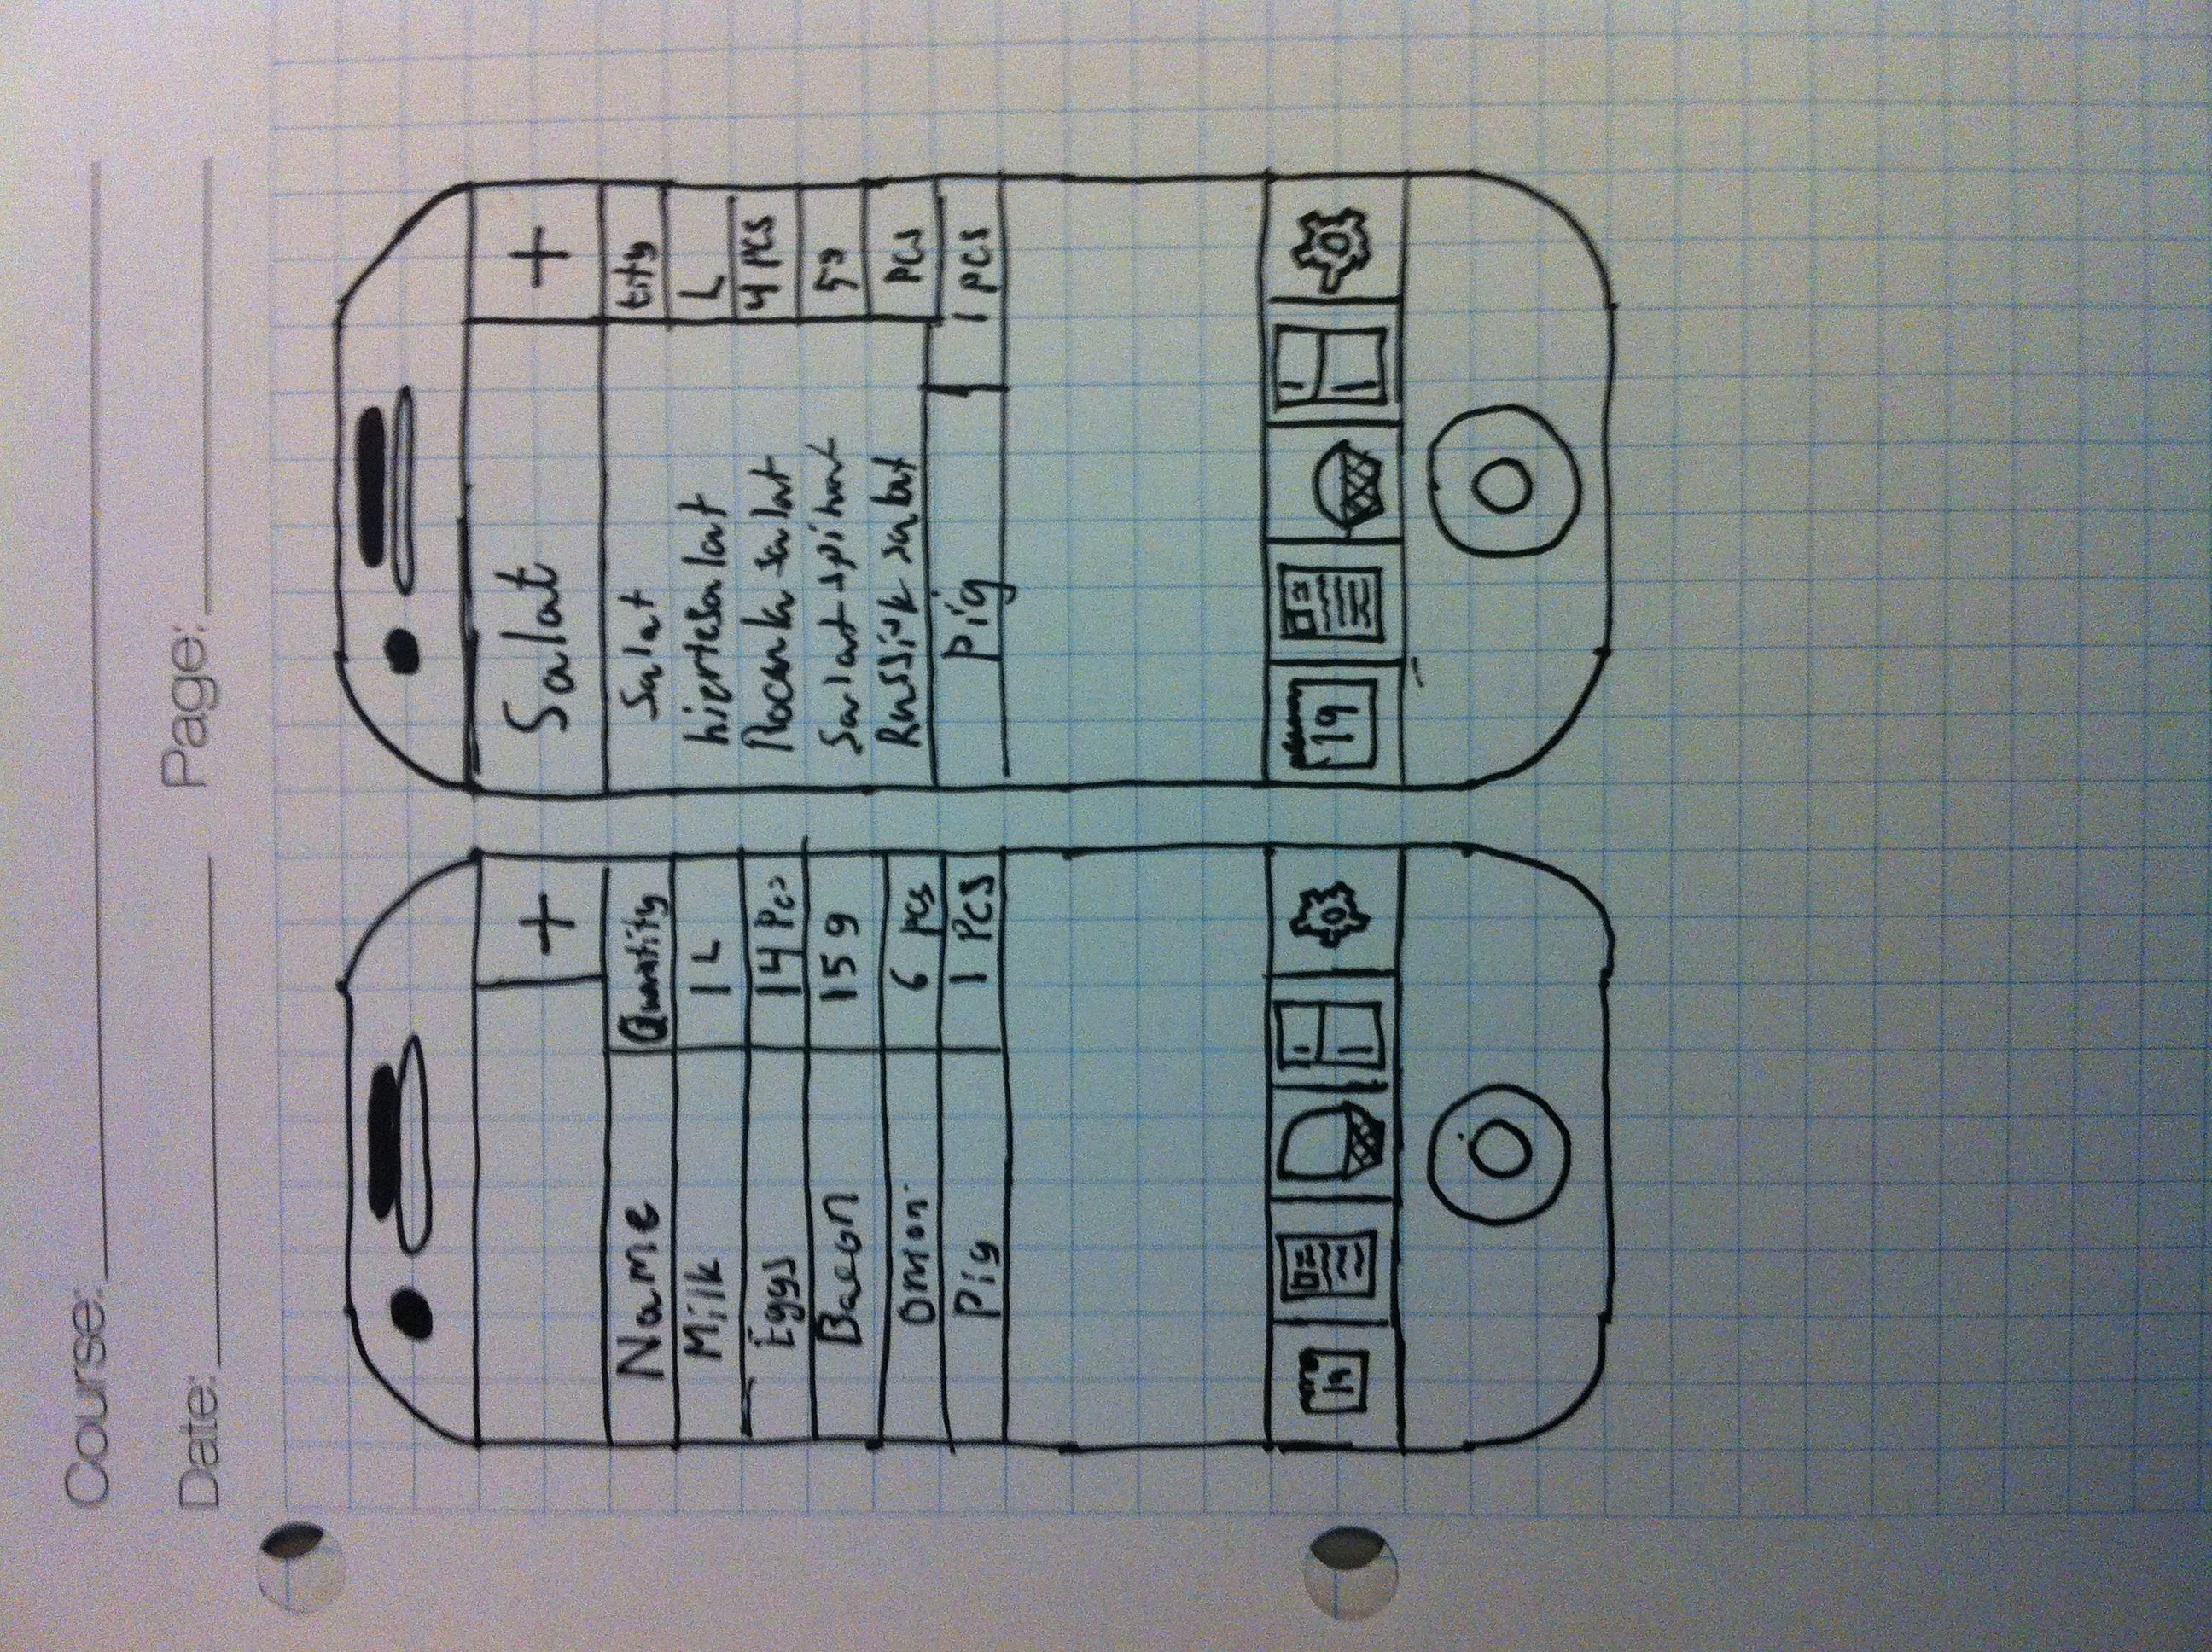
\includegraphics[width=0.5\textwidth]{Grafik/FoodPlanner/FinalShoppingListSketch}
    \caption{The final sketch of the shopping list screens}
    \label{FinalShoppingListSketch}
\end{figure}

\paragraph{Shopping List Overview screen}

The left screen in figure \ref{FinalShoppingListSketch} is the overview of the shopping list. This screen consists of two elements, not counting the general program elements, the elements is:

\begin{itemize}
	\item Search bar
	\item Table
\end{itemize}

The search bar is placed in the top of the screen, as this is where a user most likely will look for it first, because on most mobile applications and also on websites, the search bar is located at the top of the screen. The add icon is used to make the user able to add items to the inventory, that are not included in the ingredients of the meal plan.

The second element of this screen is the table, which is divided into two columns, one showing the item name, and one showing the quantity of the item. The column showing the name is broader, as the name of some items will be larger than the space needed to write the quantity.

The rows of this screens shows the ingredients on the shopping list, in the sketch, five ingredients is on the shopping list, though there could be as many as needed. If the number of different ingredients fills more than the screen can hold, the user would be able to scroll through the list by swiping upwards. Even though the user would wipe through the ingredients, the first row containing the text "Name" and "Quantity", would still be the first row.

\paragraph{Shopping List Searching Screen}

The second sketch (right sketch on \ref{FinalShoppingListSketch})  is showing the screen, when a search is performed. The screen will not change, but the search bar will expand and lay over the rest of the screen.

When a search is performed it will show a number of ingredients, in the sketch it is five, and all ingredients containing the word that have been searched for will be shown. Then the user will need to choose the ingredient they want to add to the shopping list, and click on the plus icon to add it to the list.

When a new item is added, it the user will need to go down to the quantity field, and put in the quantity of the item that will be needed.